\chapter{The First Stars}
\label{ch:first_stars}

\marginnote{
\textbf{Suggested background reading:}
\begin{itemize}
\item \href{http://adsabs.harvard.edu/abs/2013RPPh...76k2901B}{Bromm, V. 2013, Rep.~Prog.~Phys., 76, 112901}, sections 1-5 \nocite{bromm13a}
\end{itemize}
\textbf{Suggested literature:}
\begin{itemize}
\item \href{http://adsabs.harvard.edu/abs/2011ApJ...737...75G}{Greif et al., 2011, ApJ, 737, 75} \nocite{greif11a}
\end{itemize}
}

The previous chapter focused on massive stars in the present-day Universe, and in this chapter we consider how picture changes if we go back to the early Universe. The study of primordial star formation is a major topic in contemporary astrophysics, and this chapter will not provide a comprehensive review. The goal of the chapter is instead to understand how and why the picture we have outlined thus far changes in the very early Universe, and to sketch in broad outlines how the process of star formation transitioned from that found in the early Universe to that found today. The products of such early star formation are often referred to as population III stars, following the Galactic astronomy nomenclature that metal-rich disk stars like the Sun are population I and metal-poor stars found primarily in the Galactic halo, which are presumed to be older, are population II. Population III stars would then be the oldest stars, which are completely metal-free. Unlike for most other topics covered in this book, there are almost no observations that provide useful constraints on the first stars themselves -- no population III stars have ever been observed, and for reasons we discuss below it is possible that none ever will be, except perhaps via their deaths in supernova explosions. Thus this chapter will be primarily theoretical.

\section{Cosmological Context}

We begin our discussion by setting the cosmological context for the formation of the first stars. In the modern $\Lambda$CDM cosmology\footnote{For those concerned with such details: the numerical evaluations in this section are all computed for a cosmology with Hubble constant $H_0=71$ km s$^{-1}$ Mpc$^{-1}$ and densities $\Omega_b = 0.04$, $\Omega_{\rm DM} = 0.23$, and $\Omega_\Lambda = 0.73$ for baryons, dark matter, and cosmological constant, respectively.}, the Universe begins in a nearly homogenous state, with baryons and dark matter distributed nearly uniformly. The baryonic matter consists of approximately 90\% hydrogen and 10\% helium-4 (by number, not by mass), with about 1 deuterium and helium-3 per $\sim 10^5$ H atoms, and even smaller amounts of heavier elements. As the Universe expands, gravity amplifies the tiny inhomogeneities that are present. The dark matter, which dominates the mass, collapses into halos -- virialized, self-gravitating structures -- that drag the ordinary baryonic matter into them. Collapse and virialization occur when the dark matter and baryons reach a characteristic density that is $\approx 200$ times the mean density of the Universe at whatever cosmic epoch is being considered. Once halos virialize, they obey a mass-radius relation \citep{barkana01a}
\begin{equation}
R_{\rm vir} \approx 290\,\mathrm{pc} \left(\frac{M_h}{10^6\,M_\odot}\right)^{1/3} \left(\frac{1+z}{10}\right)^{-1} \left(\frac{\Delta_c}{200}\right)^{-1/3},
\end{equation}
where $M_h$ is the mass of the halo, $z$ is the redshift, and $\Delta_c$ is the overdensity of the halo after it virializes.

The dark matter is collisionless, but the baryons that fall into a halo are not. As they fall to the center of the halo they will shock, converting their gravitational potential energy to thermal energy. After they settle into hydrostatic balance, they will be in a state of virial equilibrium, with a thermal energy equal to half their gravitational potential energy. The thermal energy per particle is $\approx k_B T$, and if we equate this with half the gravitational potential energy $G M_h m_{\rm H}/R_{\rm vir}$, we obtain
\begin{equation}
T_{\rm vir} \approx \frac{G M_h m_{\rm H}}{2R_{\rm vir} k_B} \approx 900\,K 
\left(\frac{M_h}{10^6\,M_\odot}\right)^{2/3} \left(\frac{1+z}{10}\right)^{} \left(\frac{\Delta_c}{200}\right)^{1/3},
\end{equation}
where we refer to $T_{\rm vir}$ as the virial temperature. Thus gas falling into a $\sim 10^6$ $M_\odot$ dark matter halo will be shock-heated to $\approx 1000$ K. This temperature is low enough that the gas will not be ionized, and will instead remain as neutral H and He. It is in halos like this where the first stars are thought to form.


\section{Chemistry and Thermodynamics of Primordial Gas}

\subsection{The Role of H$_2$}

The temperature of $\sim 1000$ K for primordial gas falling into dark matter halos is significant, because gas at these temperatures is much too cool to produce appreciable emission from neutral hydrogen or helium.\footnote{This statement ignores the 21 cm hyperfine transition of neutral hydrogen. However, this transition has such a low emission rate, and the photons it produces are of such low energy, that it is irrelevant for cooling.} The lowest-lying excited state of H is $E = (3/4)\cdot 13.6$ eV above ground, corresponding to a temperature $T = E/k_B = 1.2\times 10^5$ K. The lowest-lying excited states of He are at similar energies. Thus there will be no significant excitation of these states in gas at temperatures of $\sim 1000$ K, and correspondingly no cooling. Since there are essentially no heavier elements in primordial gas (excepting trace amounts of Li, which also do not provide significant cooling), this means that gas falling into early, small dark matter halos cannot cool easily. This makes the situation very different from that found in present-day star forming regions, where, as we saw in chapter \ref{ch:microphysics}, gas is able to cool on timescales many orders of magnitude smaller than the dynamical time.

If the gas could not cool at all, that would be the end of the story. Gas would fall into small halos, form hydrostatic structures, and then nothing would happen. However, there is another cooling pathway to consider: formation of H$_2$ and cooling by H$_2$ radiation. The lowest lying state of H$_2$ that can radiate, the $J=2$ rotational level\footnote{Recall from chapter \ref{ch:obscold} that transitions with $\Delta J=1$ are forbidden in homonuclear molecules due to symmetry.}, is $\approx 500$ K above ground. This makes it ineffective as a coolant in the modern Universe, where CO and C$^+$ lower the temperature well below 100 K. However, in the absence of these alternatives, H$_2$ radiation potentially provides a way of cooling the gas in a primordial halo to well below the virial temperature, thereby making it possible for the gas to collapse. This route to cooling requires that H$_2$ form, and this is a challenge. Recall from our discussion of H$_2$ formation in chapter \ref{ch:microphysics} that H$_2$ formation in the gas phase is very slow due to its symmetry, which forbids electric dipole radiation. In the present-day Universe this problem is circumvented by dust grains that act as catalysts, with H$_2$ forming on their surfaces. In primordial gas, however, there are no elements capable of forming solids under interstellar conditions, and thus no grains. How can H$_2$ form under such conditions?

The answer is that an alternative catalyst is needed, and one is available: free electrons. When the Universe recombined at $z\approx 1100$, leading the emission of the cosmic microwave background, not all electrons recombined with protons to form H~\textsc{i}. A small fraction were left free. These can catalyze the formation of H$_2$ via the reaction pathway
\begin{eqnarray}
\mathrm{H} + e^- & \rightarrow & \mathrm{H}^- + h\nu \\
\mathrm{H}^- + \mathrm{H} & \rightarrow & \mathrm{H}_2 + e^-.
\end{eqnarray}
In the first step, the H captures a free electron and radiates away excess energy -- the H$^-$ binding energy is 0.77 eV \citep{weisner64a}. Since the system is not symmetric, dipole radiation is possible, and the rate coefficient, while not particularly high, is not terribly low either: $k_{-} \approx 1.1\times 10^{-16}(T/100\,\mathrm{K})^{0.88}$ cm$^3$ s$^{-1}$ \citep{glover08a}. In the second step, H$^{-}$ interacts with neutral hydrogen to form H$_2$, and the excess binding energy goes into kinetic energy of the recoiling free electron. The rate coefficient for this reaction is been measured by laboratory experiment \citep{kreckel10a}; it reaches a maximum of $k_2 \approx 4.6\times 10^{-9}$ cm$^3$ s$^{-1}$ at around 100 K, and falls gradually to $k_2\approx 2.4\times 10^{-9}$ cm$^3$ s$^{-1}$ at 1000 K and $k_2\approx 3.0\times 10^{-10}$ cm$^3$ s$^{-1}$ at $10^4$ K.

The efficiency of this formation channel depends on two factors. One obvious one is the availability of free electrons to act as catalysts. The second is the branching ratio for H$^-$ to be destroyed by forming H$_2$, rather than by the other main mechanism of H$^-$ destruction, which is photodetachment:
\begin{equation}
\mathrm{H}^- + h\nu \rightarrow \mathrm{H} + e^{-}.
\end{equation}
This mechanism is simply the inverse of the first reaction in H$_2$ formation via $e^-$ catalysis, and can occur for any photon with an energy $>0.77$ eV, the binding energy of H$^-$. At redshifts above $z\sim 100$, the cosmic microwave background is sufficiently rich in such photons that it effectively suppresses H$_2$ formation via this channel, but at lower redshifts the photodetachment rate falls, and H$_2$ formation via the H$^-$ channel becomes the dominant formation mechanism.

\subsection{Thermal and Chemical Evolution}

Armed with an understanding of how H$_2$ can form, we can now understand in rough outline the chemical and thermal processes that lead to the formation of a primordial star. These processes are summarized in Figures \ref{fig:omukai05a} and \ref{fig:omukai05b}.

\begin{figure}
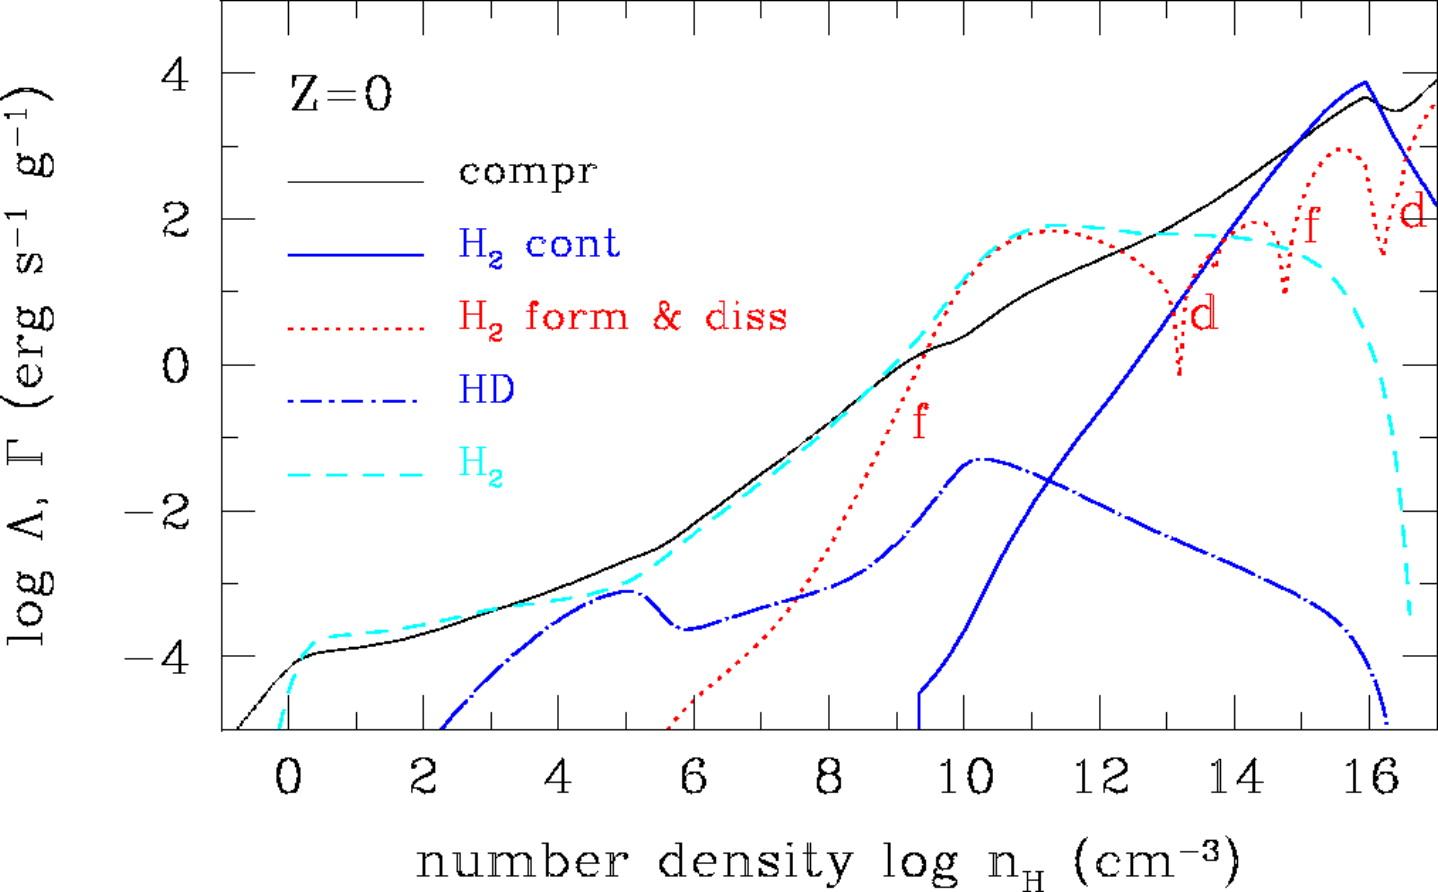
\includegraphics[width=\linewidth]{omukai05a}
\caption[Heating and cooling processes in primordial gas]{
\label{fig:omukai05a}
Results from a calculation of heating and cooling rates for processes operating in primordial gas of varying density, located at the center of a collapsing cloud. The processes included are heating by gravitational compression (black line), cooling by H$_2$ line (cyan) and continuum (solid blue) emission, cooling by HD emission (dot-dashed blue), and heating / cooling by collisional formation / dissociation of H$_2$ (dotted red). For each process, the value on the vertical axis indicates the rate of energy gain or less per unit mass per unit time. Credit: \citet{omukai05a}, \copyright AAS. Reproduced with permission.
}
\end{figure}

\begin{figure}
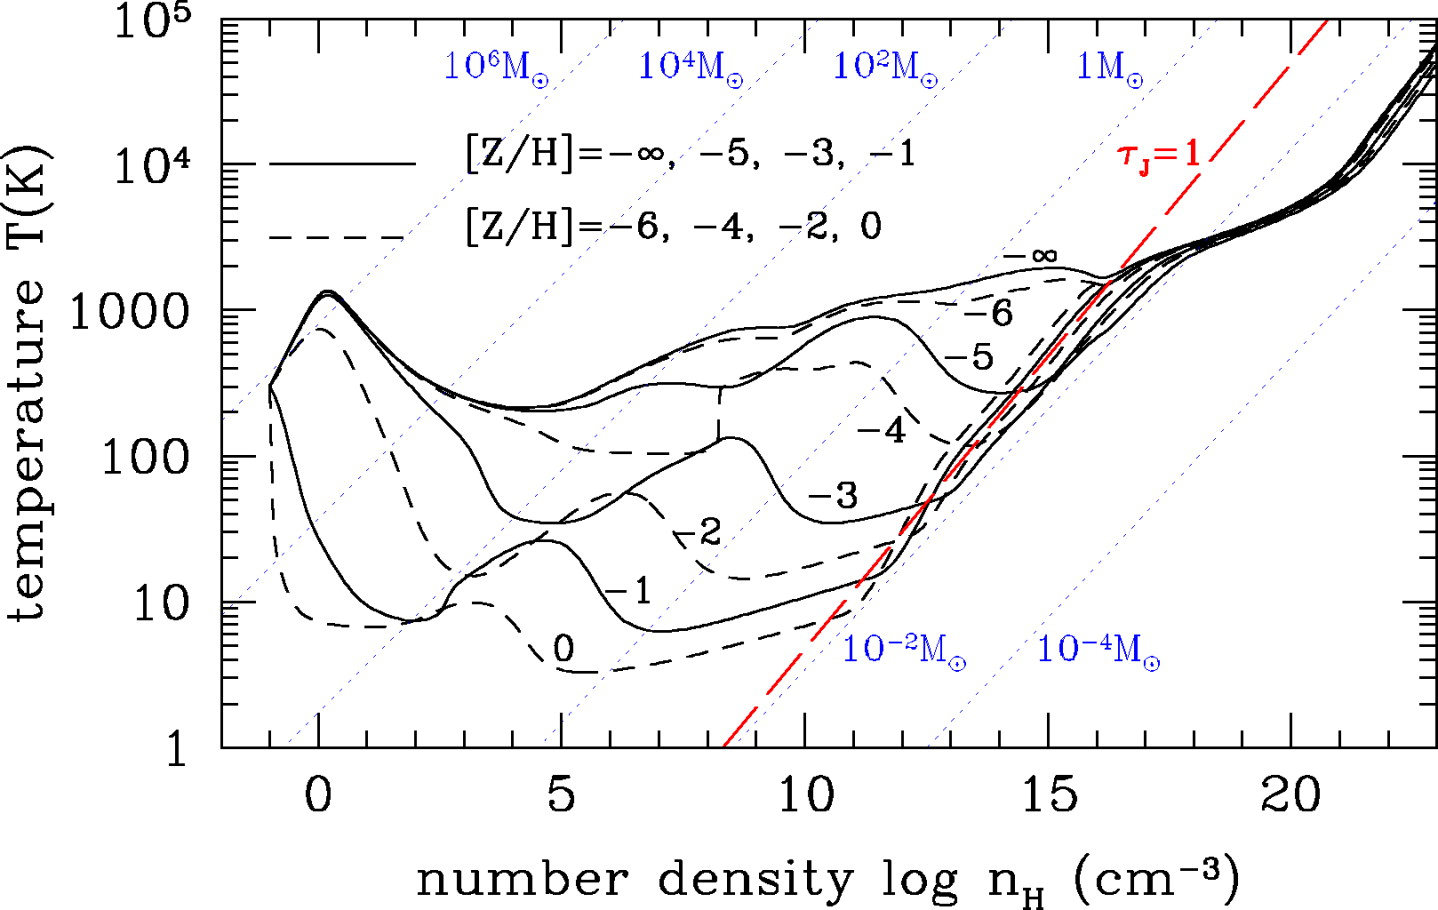
\includegraphics[width=\linewidth]{omukai05b}
\caption[Density-temperature evolution in primordial gas]{
\label{fig:omukai05b}
Density-temperature evolution of gas at the center of a collapsing cloud. Black dashed and solid lines show the trajectory of gas in the density-temperature plane, for different metallicities from primordial ($[{\rm Z}/{\rm H}] = -\infty$) to Solar ($[{\rm Z}/{\rm H}] = 0$). Dotted lines show loci of constant Jeans mass, as indicated. The red dashed line shows the point in density-temperature space where the center of the gas cloud becomes optically thick to its own cooling radiation. Credit: \citet{omukai05a}, \copyright AAS. Reproduced with permission.
}
\end{figure}

Gas enters a $\sim 10^6$ $M_\odot$ halo at $z\sim 20-30$, shocks and virializes at temperatures of thousands of K. The gas begins to form a trace amount of H$_2$ via the H$^{-}$ channel, typically no more than one H$_2$ per $\sim 10^3$ H atoms. This in turn allows the gas to cool via H$_2$ line emission. As the gas cools, its density rises to maintain approximate hydrostatic balance in the halo. This continues until the gas reaches a temperature of $\approx 200$ K, about half the temperature of the lowest-lying excited state of H$_2$ that is capable of radiating; radiation by H$_2$ cannot easily cool the gas below this point, because gas at these temperatures is too cool for collisions to excite the $J=2$ state from which radiation occurs. Cooling is also slowed by critical density effects. At low densities, as gas first begins to cool in the halo, the cooling rate per unit volume increases with density as $n^2$, because the density is below the H$_2$ critical density of $\approx 10^4$ cm$^{-3}$. Once the density exceeds this value, cooling slows to increasing with density $n$. For this reason gas tends to linger at at a density of $n\sim 10^4$ cm$^{-3}$ and a temperature $T\sim 200$ K, leading to a phase known as the loitering phase of primordial star formation. During and after the loitering phase the density gradually rises as more gas cools and compresses the densest regions that have begun to collapse. The temperature gradually rises as well, because radiative emission is unable to keep up with heating from gravitational compression.

This phase ends once the density reaches $\sim 10^8$ cm$^{-3}$. At this density, another H$_2$ formation channel appears: the three-body reaction
\begin{equation}
{\rm H} + {\rm H} + {\rm H} \rightarrow {\rm H}_2 + {\rm H}.
\end{equation}
The reaction overcomes the symmetry problem by a trick of timing. When two H atoms collide, they can temporarily form an excited compound system, but because they cannot radiate they soon separate and become unbound again. However, if while they are in this short-lived compound state they are hit by a \textit{third} hydrogen atom, they can give their excess energy to the third atom, which carries it away as kinetic energy, leaving bound H$_2$ behind. Because this process effectively requires a three-way collision, its rate varies with density as $n^3$, making it extremely density-sensitive. This is why it only becomes to be significant at densities $\sim 10^8$ cm$^{-3}$. Once the density reaches this point, however, this process rapidly increases the H$_2$ fraction from $\sim 10^{-3}$ to near unity. The exact thermal and density evolution during this phase is somewhat uncertain, as there are two competing processes. The increase in H$_2$ fraction dramatically increases the cooling rate. On the other hand, each H$_2$ formation event produces an H atom recoiling with $4.5$ eV of energy. This is quickly and efficiently thermalized, providing a strong heating source. It is unclear which of these effects dominates at densities in the range $\sim 10^8-10^{12}$ cm$^{-3}$. However, once the density reaches $n\sim 10^{12}$ cm$^{-3}$, the gas must heat up fairly strongly, because the H$_2$ lines become optically thick, suppressing further radiative cooling. At this point the evolution becomes quite similar to that in present-day star formation as discussed in chapter \ref{ch:protostar_form}.


\section{The IMF of the First Stars}

We have established that the formation of the first stars happens at characteristically much higher temperatures than the formation of present-day stars, due to the absence of cooling from metal lines. We therefore turn to the question of how this will affect the properties of the stars that result, in particular their IMF. This is a question of great importance for cosmic chemical evolution, since the nucleosynthetic yield of these first stars will depend strongly on their masses.

\subsection{Fragmentation}

\marginnote{In many ways the situation for primordial star formation is simpler than for the present-day case, and this is one of them: in chapters \ref{ch:imf_th} and \ref{ch:massivestar}, we saw that radiative feedback from stars plays a critical role in regulating the temperature evolution of the gas, and thus in regulating how it fragments. For primordial star formation this effect is substantially less important because only photons that are capable of ionizing neutral hydrogen or of exciting the Lyman-Werner transitions of H$_2$ can be absorbed by the gas, and there is no dust to absorb the remaining photons and couple them to the gas. Thus radiative heating is much less important for primordial stars than for present-day ones, though ionizing photons can be important, as will be discussed in the next section.} The first question in addressing the IMF of primordial stars is how and whether the gas from which they form will fragment. Here we can bring to bear much of the same theoretical machinery we developed in chapter \ref{ch:imf_th}. Recall that, for non-isothermal gas, we expect fragmentation to be particularly pronounced at densities and temperatures where the temperature has a minimum. Primordial gas is clearly far from isothermal as it evolves, and the most obvious minimum in Figure \ref{fig:omukai05b} is that associated with the loitering phase, at a temperature of $T\approx 200$ K and a density of $n\approx 10^4$ cm$^{-3}$, when H$_2$ cooling is suppressed because the gas is too cool to excite the $J=2$ rotational level, and because the gas is beginning to exceed the critical density of that transition. The Bonnor-Ebert mass at this density and temperature is
\begin{equation}
M_{\rm BE} = 1.18 \frac{c_s^3}{\sqrt{G^3\rho}} = 380\,M_\odot \left(\frac{T}{200\,\mathrm{K}}\right)^{3/2} \left(\frac{n}{10^4\,\mathrm{cm}^{-3}}\right)^{-1/2},
\end{equation}
where the numerical evaluation of the sound speed is for primordial gas which has a mass of $1.22m_{\rm H}=2.0\times 10^{-24}$ g per H nucleus. This high mass led most early authors working on the first stars to believe that they would be quite massive, typically more than 100 $M_\odot$.

Subsequent work has muddied this picture, and the true IMF of the first stars is still subject to extensive theoretical debate. The key question is whether the "protostellar core" produced during the loitering phase subsequently collapses monolithically or nearly so, or whether it fragments to much lower masses as it collapses. Fragmentation prior to the formation of a disk appears to be uncommon, but once a rotationally-supported accretion disk forms the situation changes, and becomes much more analogous the case of present-day massive stars discussed in chapter \ref{ch:massivestar}. The most commonly-seen outcome of fragmentation is formation of binaries with relatively large mass ratios \citep[e.g.,][]{stacy13a}. This would still leave the typical outcome of population III star formation extremely massive compared to the typical outcome of present-day star formation. On other hand, some simulations suggest that the disks fragment to produce small objects as well, some of which can be ejected via dynamical interactions \citep{clark11a, greif11a}; Figure \ref{fig:greif11a} shows an example. If this is the case, then, while some population III stars would be quite massive, others could be smaller than $1$ $M_\odot$.

While the true IMF of the first stars remains uncertain, the fact that we have never observed metal-free stars suggests that very few or none were formed with masses small enough such that they might still be in existence today. This in itself implies that the mass function was shifted to considerably higher values than what we observe today, since if the primordial IMF peaked at $\sim 0.2$ $M_\odot$ like the present one, there should be metal-free $0.2$ $M_\odot$ stars still in existence today. No such stars have been found.

\begin{figure}
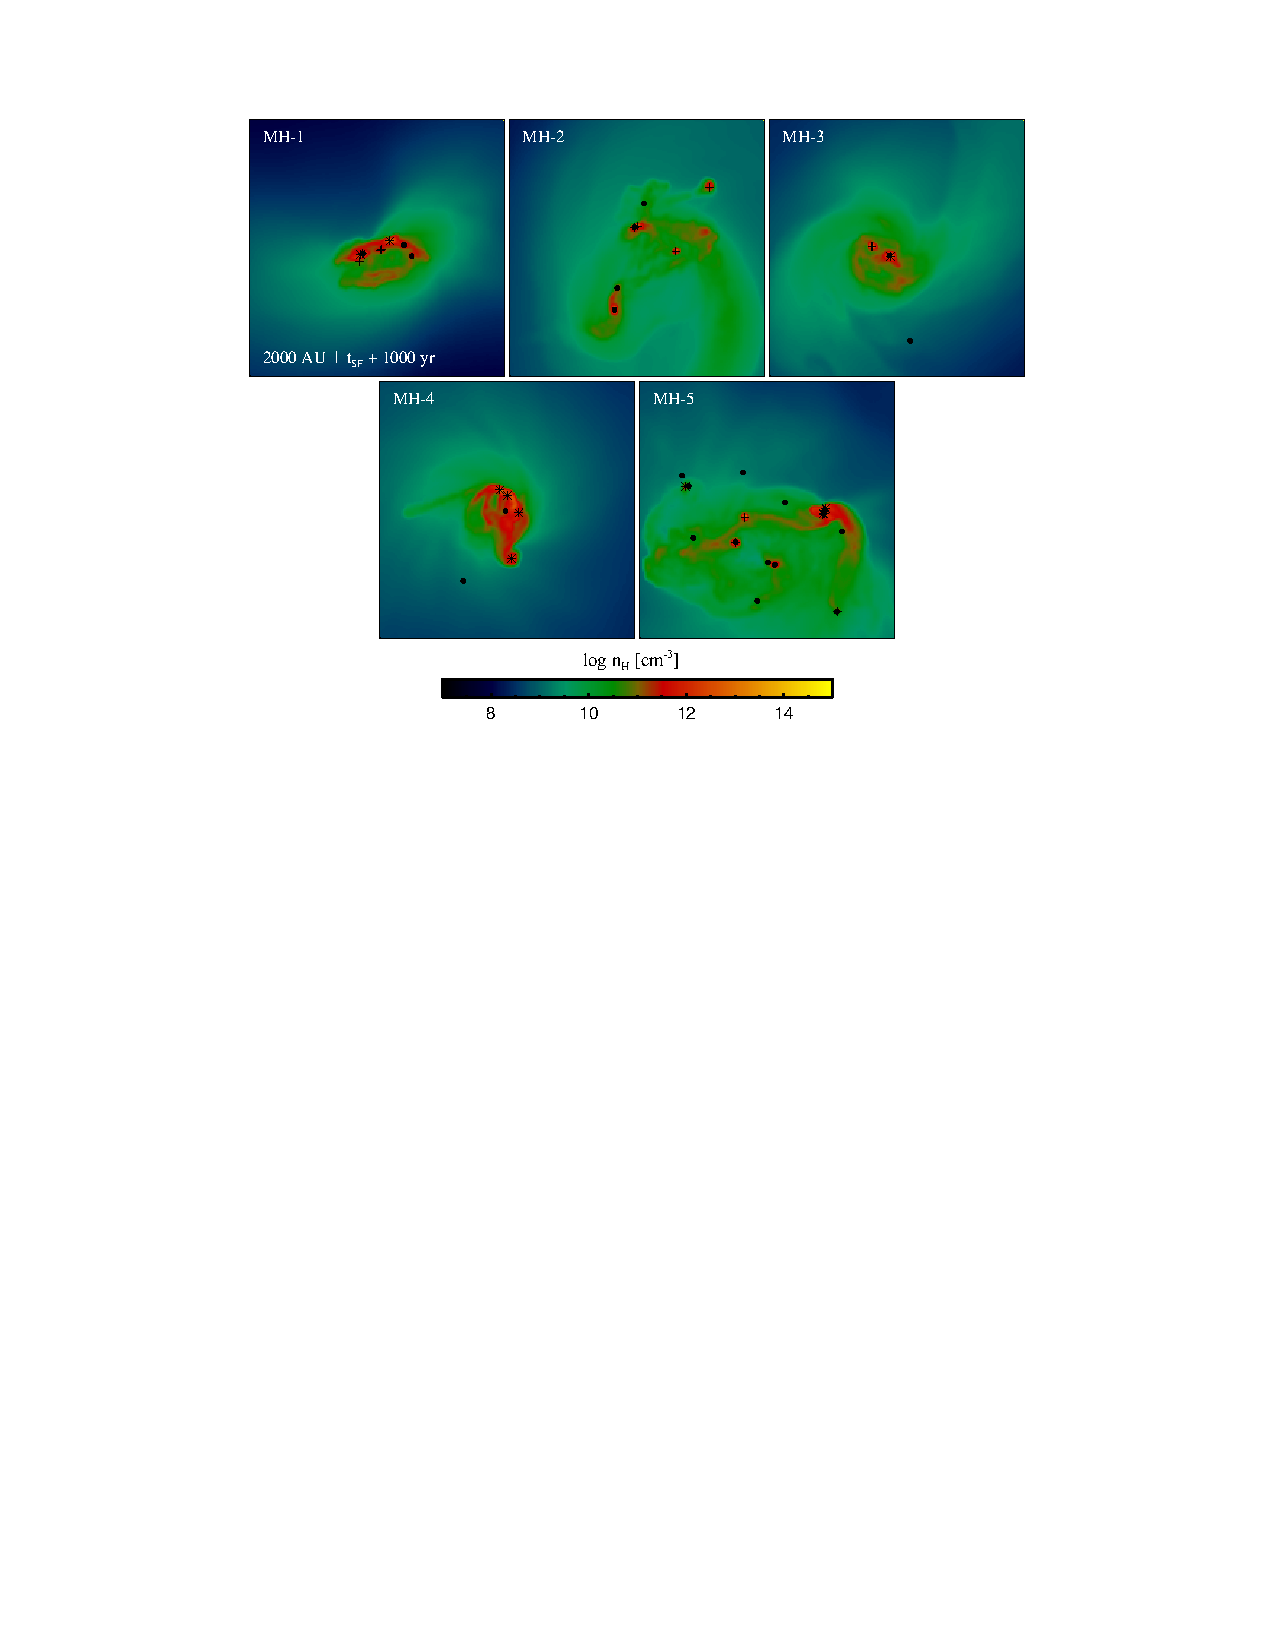
\includegraphics[width=\linewidth]{popIIIfrag_greif11}
\caption[Disk fragmentation around a primordial star]{
\label{fig:greif11a}
Results from a simulation of the formation of primordial stars. The images show the density in 2000 AU-sized regions in 5 different primordial halos, at a time 1000 years after formation of the first star in the simulation. Black dots, crosses, and stars indicate stars with masses $<1$ $M_\odot$, $1-3$ $M_\odot$, and $>3$ $M_\odot$, respectively. Credit: \citet{greif11a}, \copyright AAS. Reproduced with permission.
}
\end{figure}


\subsection{Feedback}

While the IMF of primordial stars at low masses depends largely on fragmentation, the IMF at high masses may well be shaped by feedback processes. Here it is instructive to compare to the case of present-day massive star formation. The absence of dust capable of absorbing non-ionizing photons means that radiation pressure is a somewhat smaller concern, though not a completely negligible one, since for very massive stars a significant fraction of the momentum budget of their radiation fields emerges in photons with energies above the hydrogen ionization threshold. Similarly, massive primordials stars will lack the fast radiatively-driven winds produced by present-day massive stars; such winds at driven by multiple resonant scattering of stellar photons off metal atoms in wind that have many closely-spaced levels, and primordial stars lack such atoms.

On the other hand, photoionization feedback seems likely to work for primordial stars in much the same way as it does for present-day ones, with the exception that the initial conditions for star formation are quite different. Moreover, feedback from non-ionizing photons with energies in the range $\approx 11-13.6$ eV, i.e., where they can be absorbed in the H$_2$ Lyman-Werner bands, can be significant as well. Analytic models and simulations suggest that these mechanisms might be able to evaporate the disks around primordial stars, limiting their maximum masses to tens of $M_\odot$ \citep{mckee08a, hosokawa11b, stacy12a}. The problem remains very much under investigation, however.


\section{The Transition to Modern Star Formation}

Not long after the first stars form, they will begin to change the environments around them, starting the process of transitioning to the modern mode of star formation that is the focus of the remainder of this book. The final topic in this chapter is how that transition happens.

\subsection{Ionization Evolution}

The first way that a transition away from population III star formation can occur is for the metal-free gas entering a halo to have a significantly higher abundance of electrons than the very low values expected to be be left over from the epoch of recombination. If this occurs, H$_2$ formation will occur significantly faster, the gas will cool earlier, and fragmentation to lower masses is much more likely. Stars resulting from this process are referred to as population III.2, while those formed in the truly primordial mode described above are referred to as population III.1.

An enhanced electron abundance could happen in several ways. One is for star formation to take place in gas that has already been photoionized by a population III.1 star. This seems unlikely while the population III.1 star is still shining, since its would likely heat the ionized gas to temperatures sufficient to prevent star formation. If the population III.1 star then explodes as a supernova this will pollute the gas with metals, leading to a population II star, as we discuss below. On the other hand, if the population III.1 star instead collapses directly to a black hole, without dispersing any metals, then any gas remaining in its halo would be ripe for population III.2 star formation.

\subsection{Chemical Evolution}
\label{ssec:chemevol}

Once a population III.1 or III.2 star explodes as a supernova, it disperses metals into the surrounding ISM, triggering a transition from population III to population II star formation. An outstanding question in this field is what level of metal enrichment is sufficient to produce this transition. Observationally, as of this writing, the most carbon-poor known star has a carbon abundance $\approx 4.5 \times 10^{-5}$ times that of the Sun \citep{caffau11a}, while the most iron-poor contains $<10^{-7}$ of the Solar iron abundance \citep{keller14a}. That both stars continue to exist today implies that it must be possible to from stars with masses well under $1$ $M_\odot$ with such low chemical abundances. In discussing this, it is helpful to consider two roles that metals have played in our discussion thus far. First, metals in the gas phase provide an important coolant for the ISM, allowing gas to cool on less than a dynamical timescale. Second, metals in the form of dust grains provide cooling at high densities where the dust and gas become collisionally-coupled, and also provide surfaces to catalyze chemical reactions, particularly H$_2$ formation.

\paragraph{Metal Line Cooling}

The distinguishing characteristic of modern star formation is the ability of star-forming gas to cool much faster than a dynamical time. Metal line cooling becomes significant when there are enough metals to make this possible, at which point they supplant H$_2$ cooling and trigger a transition to a more modern star formation mode. We can analytically estimate the metallicity required to achieve this, following the original calculation by \citet{bromm01a}, by comparing the rate of metal line cooling to the rate of heating due to adiabatic compression that we expect for baryons at the center of a virialized dark matter halo.

The calculation here is quite analogous to the one presented in Section \ref{ssec:iso_adiabat}. We
let $e$ be the thermal energy per unit mass of a particular gas parcel, and let $\Gamma$ and $\Lambda$ be the rates of change in $e$ due to heating and cooling processes, so
\begin{equation}
\frac{de}{dt} = \Gamma - \Lambda.
\end{equation}
The heating rate due to adiabatic compression is no different in the primordial case than in the present-day one: $\Gamma = -p\, (d/dt) (1/\rho) \approx -p/(\rho t_{\rm ff})$. For $t_{\rm ff} = \sqrt{3\pi/32G\rho}$, we have
\begin{equation}
\label{eq:gamma_ad_firststar}
\Gamma \approx k_B T \sqrt{\frac{32 G n}{3\pi \mu m_{\rm H}}},
\end{equation}
where $n$ is the number density of H nuclei and $\mu$ is the mean mass per H nucleus in units of $m_{\rm H}$; for near-primordial composition $\mu = 1.22$.

We must compare this to the rate of cooling due to metal lines. In the very metal-poor gas with which we are concerned, we do not expect appreciable numbers of CO or other heavy molecules to form, due to both absence of dust shielding and the long timescales required for chemical reactions when the constituent atoms are scarce. We must therefore consider cooling via atomic lines. The two most important cooling species are C$^+$ and O.\footnote{Recall from Section \ref{ssec:cochemistry} that carbon is primarily ionized under interstellar conditions because its ionization potential is smaller than that of hydrogen; in contrast, O has a higher ionization potential than H, and is largely neutral.} The former provides cooling mainly through its $158$ $\mu$m fine structure line, while the latter cools via a pair of lines at 63 and 145 $\mu$m. These transitions are generally optically thin, and their critical densities are high enough that we can treat them as being in the low-density limit. Recalling the discussion in Section \ref{ssec:molecular_lines}, and in particular Equation \ref{eq:cool_lowden}, the rate of cooling per unit mass in this limit can be written as
\begin{equation}
\Lambda = \frac{1}{\rho}n_X E A e^{-E/k_BT} \frac{n}{n_{\rm crit}} = \frac{n_X E k_{u\ell}}{\mu m_{\rm H}} e^{-E/k_B T},
\end{equation}
where here $n_X$ is the number density of the cooling species (either C$^+$ or O), $n$ is the number density of the primary collision partner (atomic hydrogen), $E$ is the energy of the cooling level, $A$ is the Einstein $A$ for the transition, $k_{u\ell}$ is the collisional de-excitation rate from the upper to the lower level, and $T$ is the temperature. Note that, in the second equality, the value of the Einstein coefficient and the number density of H have both dropped out. This is as we should expect: at low densities, cooling occurs when a hydrogen atom collides with a metal atom and excites it; the metal atom then radiates long before its next collision. Consequently, the cooling rate does not depend on exactly how long the metal atom takes to radiate (the Einstein $A$ coefficient), only on the timescale between H atoms colliding with other atoms (hence the dependence on $n_X$ but not on $n$), the collisional excitation probability (the factor $k_{u\ell} e^{-E/k_B T}$), and the energy lost per excitation ($E$).

For the lines with which we are concerned, $E/k_B = 91$ K, 228 K, and 327 K for the C$^+$ 158 $\mu$m, O 63 $\mu$m, and O 145 $\mu$m lines, respectively. The corresponding collisional de-excitation rate coefficients for collisions with H are $k_{u\ell}\approx 8\times 10^{-10}$, $5\times 10^{-10}$, and $7\times 10^{-10}$ cm$^3$ s$^{-1}$ at temperatures $\sim 1000$ K.\footnote{These rate coefficients are taken from the \href{http://home.strw.leidenuniv.nl/~moldata/}{Leiden Atomic and Molecular Database} -- \citet{schoier05a}; original data are from \citet{launay77a} and \citet{barinovs05a} for C$^+$, and from \citet{abrahamsson07a} for O.} For simplicity, let us assume that the C and O abundances are simply given by their Milky Way values scaled by a metallicity factor; specifically, we can take $n_{\rm C}/n = 2\times 10^{-4} Z'$ and $n_{\rm O}/n = 4\times 10^{-4} Z'$, where $Z'$ is the metallicity normalized to Solar. Finally, let us adopt a temperature $T \gg 300$ K, so that we can treat the $e^{-E/k_B T}$ factors for all three lines as unity; this is not strictly true, but for a rough estimate it is sufficient. Under these assumptions, and plugging in the quantities given above, we can write the cooling rate as
\begin{equation}
\Lambda = \Lambda_0 n Z',
\end{equation}
with $\Lambda_0 \approx 0.01$ erg cm$^3$ g$^{-1}$ s$^{-1}$.

Equating the heating rate $\Gamma$ and the cooling rate $\Lambda$, we find that metal-induced radiative cooling is able to match heating when
\begin{equation}
Z' = \frac{k_B T}{\Lambda_0} \sqrt{\frac{32 G}{3\pi \mu m_{\rm H} n}} = 4.5\times 10^{-4} \left(\frac{T}{1000\,\mathrm{K}}\right)\left(\frac{n}{100\,\mathrm{cm}^{-3}}\right)^{-1/2}.
\end{equation}
For the numerical evaluation we have plugged in typical densities and temperatures near the centers of virialized halos with mass $\sim 10^6$ $M_\odot$. Thus we expect that metal line cooling will become significant above metallicities of $Z'\sim 10^{-3.5}$.


\paragraph{Dust Effects}

The second channel through which metals affect the behavior of interstellar gas is by forming dust grains, which can serve as both radiators and chemical catalysts for the formation of molecules, particularly H$_2$. We defer the question of when dust becomes important as a catalyst to problem set 5, and here focus on the role of dust as a radiator. Dust is particularly important in this role because dust grains, as solid particles, can emit continuum radiation rather than being limited to emission at particular frequencies. This makes them much more efficient than gas at coupling to a radiation field, either via emission or absorption. In our discussion of the IMF and massive stars in chapters \ref{ch:imf_th} and \ref{ch:massivestar}, we focused on the latter effect, but before star formation begins in a region and produces a significant radiation field to absorb, the former effect is more important. Dust provides a potential mechanism to cool interstellar gas far beyond what would be possible with either H$_2$ or atomic line emission.

Because dust is such an efficient radiator, the bottleneck in dust cooling of the gas is usually the rate at which energy can be transmitted from the gas to the dust via collisions, not the rate at which dust can radiate it (though this can cease to be true if the dust becomes optically thick.) The grain-gas transfer rate in turn is limited by the total cross sectional area of dust grains available for collision. Since collisions are fastest when the density is high, we will focus on a high density regime when the gas has been fully converted to H$_2$, if only by three-body reactions occurring in the gas phase. To compute when dust cooling becomes important, let us consider a simplified problem\footnote{A more complete treatment of this problem may be found in \citet{schneider06a} and \citet{schneider12a}.}: suppose that we have a population of spherical dust grains with radius $a$, floating in a sea of hydrogen molecules with temperature $T$ and number density $n$. Since the velocities are grains are generally much smaller than those of individual hydrogen atoms, we can consider the grains at rest. We expect the rate at which hydrogen atoms strike a single dust grain to be of order $n\sigma v$, where $\sigma \approx \pi a^2$ is the grain cross section and $v\approx \sqrt{kT/\mu m_{\rm H}}$ is the thermal velocity of the particles; for fully-molecular gas of primordial composition, $\mu \approx 2.3$. Detailed integration over a Maxwellian distribution of gas velocities \citep{draine11a} gives a collision rate per grain
\begin{equation}
\mbox{collision rate / grain} = n \sqrt{\frac{8 k_B T}{\pi \mu m_{\rm H}}} \pi a^2,
\end{equation}
in line with this expectation.

The rate of collisions per unit gas mass is simply this multiplied by the number of dust grains per unit total (gas plus dust) mass. Let $m_{\rm gr}$ be the mass per grain, and let $\mathcal{D}$ be the ratio of dust mass to gas mass density, i.e., for every 1 g of gas, there are $\mathcal{D}$ g of dust present. Thus the rate of grain-gas collisions per unit mass is given by
\begin{equation}
\mbox{collision rate / mass} =  n \sqrt{\frac{8 k_B T}{\pi \mu m_{\rm H}}} \pi a^2 \left(\frac{\mathcal{D}}{m_{\rm gr}}\right)
\equiv n \mathcal{D} \sqrt{\frac{8 k_B T}{\pi \mu m_{\rm H}}} \mathcal{S}
\end{equation}
where we have defined the quantity $\mathcal{S} = \pi a^2/m_{\rm gr}$ as the dust cross section per unit dust mass, which is a function only of the grains themselves (their density, composition, geometry, etc.) and not of their abundance. The value of $\mathcal{S}$ is quite uncertain; we have a reasonable estimate of it for present-day interstellar dust, but it is likely to be quite different for the case relevant for the population III to population II transition, because at such early times any grains present are probably those that have condensed directly out of supernova ejecta, rather than the mix of grains produced by supernovae, AGB and red giant stars, and \textit{in situ} processing in the interstellar medium that exists in the present-day Universe. \citet{schneider12a} suggest values $\mathcal{S} \sim 10^5$ cm$^2$ g$^{-1}$, but this should be taken with considerable caution.

The rate of energy transfer should be proportional to this rate times the mean energy transfer per collision. Again integrating over a Maxwellian distribution of hydrogen atom velocities, the mean energy per hydrogen atom striking the grain is $2k_B T.$\footnote{The value $2k_B T$ is slightly higher than the canonical $(3/2) k_B T$ per particle in a Maxwellian distribution because faster-moving hydrogen atoms are more likely to collide with a grain, and thus the average kinetic energy of colliding particles is slightly higher than the average kinetic energy of all particles.}  If grain-gas collisions were perfectly elastic then there would be no energy transfer between the two, and if it were perfectly inelastic then the net energy transfer would be $2k_B T$ in the limit where the dust temperature $T_d \ll T$. We interpolate between these two extremes by writing the mean energy transfer per dust-gas collision as
\begin{equation}
\left\langle\Delta E\right\rangle = 2\alpha k_B (T - T_d),
\end{equation}
where $\alpha = 0$ corresponds to perfect elasticity, $\alpha=1$ to perfect inelasticity, and we have written the temperature dependence as proportional to $T-T_d$ to properly capture the effect that energy should flow from gas to trains for $T > T_d$ and from grains to gas for $T < T_d$, and that there should be no net energy transfer if $T=T_d$. The quantity $\alpha$ is known as the accommodation coefficient, and laboratory measurements and theoretical calculations suggest that it is of order $\sim 0.5$.

Putting this together, the rate of energy transfer from gas to grains per unit gas mass, and thus the rate of dust cooling, will be given by
\begin{equation}
\Lambda = 2 \alpha n \mathcal{D} \mathcal{S} \sqrt{\frac{8 k_B T}{\pi \mu m_{\rm H}}} k_B (T-T_d).
\end{equation}
If we now equate this cooling rate with the heating rate derived above (equation \ref{eq:gamma_ad_firststar}), we find that they become equal at a dust-to-gas ratio
\begin{equation}
\mathcal{D} = \frac{1}{\alpha \mathcal{S}} \sqrt{\frac{G}{3 n k_B T}}
\end{equation}
where for simplicity we have assumed $T \gg T_d$.

For dust cooling to be effective, it must kick in before the system becomes completely optically thick at a density $n\sim 10^{12}$ cm$^{-3}$. Thus to get the minimum value of $\mathcal{D}$ for which dust cooling matters, we will use this value of $n$. Consulting the zero-metallicity case shown in Figure \ref{fig:omukai05b}, the temperature at this density range is $T\sim 1000$ K. Plugging in these values, along with the fiducial values of $\alpha$ and $\mathcal{S}$ discussed above, we have
\begin{equation}
\mathcal{D} \approx 8\times 10^{-9}\left(\frac{0.5}{\alpha}\right)
\left(\frac{10^5\mbox{ cm}^2\mbox{ g}^{-1}}{\mathcal{S}}\right)
\left(\frac{n}{10^{12}\mbox{ cm}^{-3}}\right)^{-1/2} \left(\frac{T}{1000\mbox{ K}}\right)^{-1/2},
\end{equation}
or about $10^6$ times smaller than the Solar neighborhood value $\mathcal{D} \approx 0.01$. A further complication in making use of this value is that this estimate is phrased in terms of the dust to gas ratio, but we have little idea how to translate this into a metallicity, which is the quantity that we can measure in surviving stars. The dust-to-metals ratio in the present-day Universe is a result of a competition between grain production in supernovae and evolved stars and grain destruction (and possibly also grain growth) in the interstellar medium. It is observed to be roughly constant down to metallicities of $\sim 10\%$ of Solar, but to fall decrease below that \citep{remy-ruyer14a}. At the time of the transition from primordial to modern star formation, supernovae will have occurred, but it is not clear which other processes might have, and there is no observational guidance to be had.


